% THIS IS SIGPROC-SP.TEX - VERSION 3.1
% WORKS WITH V3.2SP OF ACM_PROC_ARTICLE-SP.CLS
% APRIL 2009
%
% It is an example file showing how to use the 'acm_proc_article-sp.cls' V3.2SP
% LaTeX2e document class file for Conference Proceedings submissions.
% ----------------------------------------------------------------------------------------------------------------
% This .tex file (and associated .cls V3.2SP) *DOES NOT* produce:
%       1) The Permission Statement
%       2) The Conference (location) Info information
%       3) The Copyright Line with ACM data
%       4) Page numbering
% ---------------------------------------------------------------------------------------------------------------
% It is an example which *does* use the .bib file (from which the .bbl file
% is produced).
% REMEMBER HOWEVER: After having produced the .bbl file,
% and prior to final submission,
% you need to 'insert'  your .bbl file into your source .tex file so as to provide
% ONE 'self-contained' source file.
%
% Questions regarding SIGS should be sent to
% Adrienne Griscti ---> griscti@acm.org
%
% Questions/suggestions regarding the guidelines, .tex and .cls files, etc. to
% Gerald Murray ---> murray@hq.acm.org
%
% For tracking purposes - this is V3.1SP - APRIL 2009

%Old document Class 
%\documentclass[a4paper]{acm_proc_article-sp}
\documentclass{sig-alternate}
%\usepackage[margin=1in]{geometry}
\usepackage{amsmath}
\usepackage{url}
\usepackage{graphicx}
\usepackage{alltt}
\usepackage{algorithm}

\usepackage{algorithmic}
\usepackage{cite}
\usepackage{flushend}
\usepackage{tabularx}

%\lstset{language=C}
\usepackage{times}
\usepackage{graphicx}
\usepackage{epsf}
\usepackage{verbatim}
\usepackage{psfig}
\usepackage{cite}
\usepackage{url}
\usepackage{color}
\usepackage{alltt}

\usepackage{longtable,lscape}
\usepackage{slashbox,multirow}
\usepackage{colortbl}
\usepackage{mathrsfs}

\newcommand{\Add}{\CodeIn{add}}
\newcommand{\AVTree}{\CodeIn{AVTree}}
\newcommand{\Assignment}[3]{$\langle$ \Object{#1}, \Object{#2}, \Object{#3} $\rangle$}
\newcommand{\BinaryTreeRemove}{\CodeIn{BinaryTree\_remove}}
\newcommand{\BinaryTree}{\CodeIn{BinaryTree}}
\newcommand{\Caption}{\caption}
\newcommand{\Char}[1]{`#1'}
\newcommand{\CheckRep}{\CodeIn{checkRep}}
\newcommand{\ClassC}{\CodeIn{C}}
\newcommand{\CodeIn}[1]{{\small\texttt{#1}}}
\newcommand{\CodeOutSize}{\scriptsize}
\newcommand{\Comment}[1]{}
\newcommand{\Ensures}{\CodeIn{ensures}}
\newcommand{\ExtractMax}{\CodeIn{extractMax}}
\newcommand{\FAL}{field-ordering}
\newcommand{\FALs}{field-orderings}
\newcommand{\Fact}{observation}
\newcommand{\Get}{\CodeIn{get}}
\newcommand{\HashSet}{\CodeIn{HashSet}}
\newcommand{\HeapArray}{\CodeIn{HeapArray}}
\newcommand{\Intro}[1]{\emph{#1}}
\newcommand{\Invariant}{\CodeIn{invariant}}
\newcommand{\JUC}{\CodeIn{java.\-util.\-Collections}}
\newcommand{\JUS}{\CodeIn{java.\-util.\-Set}}
\newcommand{\JUTM}{\CodeIn{java.\-util.\-TreeMap}}
\newcommand{\JUTS}{\CodeIn{java.\-util.\-TreeSet}}
\newcommand{\JUV}{\CodeIn{java.\-util.\-Vector}}
\newcommand{\JMLPlusJUnit}{JML+JUnit}
\newcommand{\Korat}{Korat}
\newcommand{\Left}{\CodeIn{left}}
\newcommand{\Lookup}{\CodeIn{lookup}}
\newcommand{\MethM}{\CodeIn{m}}
\newcommand{\Node}[1]{\CodeIn{N}$_#1$}
\newcommand{\Null}{\CodeIn{null}}
\newcommand{\Object}[1]{\CodeIn{o}\ensuremath{_#1}}
\newcommand{\PostM}{\MethM$_{post}$}
\newcommand{\PreM}{\MethM$_{pre}$}
\newcommand{\Put}{\CodeIn{put}}
\newcommand{\Remove}{\CodeIn{remove}}
\newcommand{\RepOk}{\CodeIn{repOk}}
\newcommand{\Requires}{\CodeIn{requires}}
\newcommand{\Reverse}{\CodeIn{reverse}}
\newcommand{\Right}{\CodeIn{right}}
\newcommand{\Root}{\CodeIn{root}}
\newcommand{\Set}{\CodeIn{set}}
\newcommand{\State}[1]{2^{#1}}
\newcommand{\TestEra}{TestEra}
\newcommand{\TreeMap}{\CodeIn{TreeMap}}

\newenvironment{CodeOut}{\begin{scriptsize}}{\end{scriptsize}}
\newenvironment{SmallOut}{\begin{small}}{\end{small}}

\newcommand{\pairwiseEquals}{PairwiseEquals}
\newcommand{\monitorEquals}{MonitorEquals}
%\newcommand{\monitorWField}{WholeStateW}
\newcommand{\traverseField}{WholeState}
\newcommand{\monitorSMSeq}{ModifyingSeq}
\newcommand{\monitorSeq}{WholeSeq}

\newcommand{\IntStack}{\CodeIn{IntStack}}
\newcommand{\UBStack}{\CodeIn{UBStack}}
\newcommand{\BSet}{\CodeIn{BSet}}
\newcommand{\BBag}{\CodeIn{BBag}}
\newcommand{\ShoppingCart}{\CodeIn{ShoppingCart}}
\newcommand{\BankAccount}{\CodeIn{BankAccount}}
\newcommand{\BinarySearchTree}{\CodeIn{BinarySearchTree}}
\newcommand{\LinkedList}{\CodeIn{LinkedList}}

\newcommand{\Book}{\CodeIn{Book}}
\newcommand{\Library}{\CodeIn{Library}}

\newcommand{\Jtest}{Jtest}
\newcommand{\JCrasher}{JCrasher}
\newcommand{\Daikon}{Daikon}
\newcommand{\JUnit}{JUnit}

\newcommand{\trie}{trie}

\newcommand{\Perl}{Perl}


\newcommand{\SubjectCount}{11}
\newcommand{\DSSubjectCount}{two}

\newcommand{\Equals}{\CodeIn{equals}}
\newcommand{\Pairwise}{PairwiseEquals}
\newcommand{\Subgraph}{MonitorEquals}
\newcommand{\Concrete}{WholeState}
\newcommand{\ModSeq}{ModifyingSeq}
\newcommand{\Seq}{WholeSeq}
\newcommand{\Aeq}{equality}

\newcommand{\Meaning}[1]{\ensuremath{[\![}#1\ensuremath{]\!]}}
\newcommand{\Pair}[2]{\ensuremath{\langle #1, #2 \rangle}}
\newcommand{\Triple}[3]{\ensuremath{\langle #1, #2, #3 \rangle}}
\newcommand{\SetSuch}[2]{\ensuremath{\{ #1 | #2 \}}}

\newcommand{\Equiv}[2]{\ensuremath{#1 \EquivSTRel{} #2}}
\newcommand{\EquivME}{\Equiv}
\newcommand{\EquivST}{\Equiv}
\newcommand{\EquivSTRel}{\ensuremath{\cong}}
\newcommand{\Redundant}[2]{\ensuremath{#1 \lhd #2}}
\newcommand{\VB}{\ensuremath{\mid}}
\newcommand{\MES}{method-entry state}

\newcommand{\Small}[1]{{\small{#1}}}

\newcommand{\CenterCell}[1]{\multicolumn{1}{c|}{#1}}


%\addtolength{\topmargin}{.825in}

\newcommand{\tool}{{\sc ICON}}
\newcommand{\amazon}{\CodeIn{Amazon S3 REST} API developer documentation}
\newcommand{\amazonAPI}{\CodeIn{Amazon S3 REST} API}
\newcommand{\paypalAPI}{\CodeIn{Paypal REST} API}

\begin{document}
%
% --- Author Metadata here ---
%\conferenceinfo{FSE}{'14 Hong Kong}
%\CopyrightYear{2007} % Allows default copyright year (20XX) to be over-ridden - IF NEED BE.
%\crdata{0-12345-67-8/90/01}  % Allows default copyright data (0-89791-88-6/97/05) to be over-ridden - IF NEED BE.
% --- End of Author Metadata ---

\title{{\ttlit ICON}: {\ttlit I}nferring Temporal {\ttlit Con}straints from Natural Language API Descriptions}
%\subtitle{[Extended Abstract]
%\titlenote{A full version of this paper is available as
%\textit{Author's Guide to Preparing ACM SIG Proceedings Using
%\LaTeX$2_\epsilon$\ and BibTeX} at
%\texttt{www.acm.org/eaddress.htm}}}
%
% You need the command \numberofauthors to handle the 'placement
% and alignment' of the authors beneath the title.
%
% For aesthetic reasons, we recommend 'three authors at a time'
% i.e. three 'name/affiliation blocks' be placed beneath the title.
%
% NOTE: You are NOT restricted in how many 'rows' of
% "name/affiliations" may appear. We just ask that you restrict
% the number of 'columns' to three.
%
% Because of the available 'opening page real-estate'
% we ask you to refrain from putting more than six authors
% (two rows with three columns) beneath the article title.
% More than six makes the first-page appear very cluttered indeed.
%
% Use the \alignauthor commands to handle the names
% and affiliations for an 'aesthetic maximum' of six authors.
% Add names, affiliations, addresses for
% the seventh etc. author(s) as the argument for the
% \additionalauthors command.
% These 'additional authors' will be output/set for you
% without further effort on your part as the last section in
% the body of your article BEFORE References or any Appendices.

\numberofauthors{1} %  in this sample file, there are a *total*
% of EIGHT authors. SIX appear on the 'first-page' (for formatting
% reasons) and the remaining two appear in the \additionalauthors section.
%
\author{
% You can go ahead and credit any number of authors here,
% e.g. one 'row of three' or two rows (consisting of one row of three
% and a second row of one, two or three).
%
% The command \alignauthor (no curly braces needed) should
% precede each author name, affiliation/snail-mail address and
% e-mail address. Additionally, tag each line of
% affiliation/address with \affaddr, and tag the
% e-mail address with \email.
%
% 1st. author
\alignauthor
Rahul Pandita$^1$, Kunal Taneja$^2$, Tao Xie$^3$, Laurie Williams$^1$, Teresa Tung$^2$\\%\titlenote{Dr.~Trovato insisted his name be first.}\\
       \affaddr{$^1$Department of Computer Science, North Carolina State University, Raleigh, NC, USA}\\
       \affaddr{$^2$Accenture Technology Labs, San Jose, CA, USA}\\
       \affaddr{$^3$Department of Computer Science, University of Illinois, Urbana-Champaign, IL, USA}\\
       \email{{\normalsize rpandit@ncsu.edu, k.a.taneja@accenture.com, taoxie@illinois.edu, williams@csc.ncsu.edu, teresa.tung@accenture.com}}
% 2nd. author
%\alignauthor
%Kunal Taneja\\
%	   %\titlenote{The secretary disavows any knowledge of this author's actions.}\\
%       \affaddr{Accenture Technology Labs}\\
%       \affaddr{San Jose, CA, USA}\\
%       \email{k.a.taneja@accenture.com}
%% 3rd. author
%\alignauthor 
%Tao Xie\\
%	   %\titlenote{This author is the one who did all the really hard work.}\\
%       %\affaddr{Department of Computer Science}\\
%       \affaddr{University of Illinois}\\
%       \affaddr{Urbana-Champaign, IL, USA}\\
%       \email{taoxie@illinois.edu}
%\and  % use '\and' if you need 'another row' of author names
%% 4th. author
%\alignauthor Laurie Williams\\
%       %\affaddr{Department of Computer Science}\\
%       \affaddr{North Carolina State University}\\
%       \affaddr{Raleigh, NC, USA}\\
%       \email{williams@csc.ncsu.edu}
%% 5th. author
%\alignauthor Teresa Tung\\
%       \affaddr{Accenture Technology Labs}\\
%       \affaddr{San Jose, CA, USA}\\
%       \email{teresa.tung@accenture.com}
}
% There's nothing stopping you putting the seventh, eighth, etc.
% author on the opening page (as the 'third row') but we ask,
% for aesthetic reasons that you place these 'additional authors'
% in the \additional authors block, viz.
%\additionalauthors{Additional authors: John Smith (The Th{\o}rv{\"a}ld Group,
%email: {\texttt{jsmith@affiliation.org}}) and Julius P.~Kumquat
%(The Kumquat Consortium, email: {\texttt{jpkumquat@consortium.net}}).}
\date{30 July 1999}
% Just remember to make sure that the TOTAL number of authors
% is the number that will appear on the first page PLUS the
% number that will appear in the \additionalauthors section.

\maketitle
\begin{abstract}
Formal specifications of an Application Programming Interface (API) usage are highly desirable,
because they are the precursor to the formal analysis tools such as model checkers and runtime verifiers.
However, most API's do not have formal specifications.
In contrast documentation of methods contain detailed specifications of the usage in natural language text.
However, formal analysis tools are not designed to work on specifications in natural languages.
Manually writing formal specifications based on natural language text in API documents can be prohibitively time consuming and error prone.
To address this issue, we propose a natural language processing based novel approach \tool\ to precisely infer constraints from natural language text of API documents.
In particular, we focus on temporal constraints, that are defined as constraints on the
\textit{allowed sequence of invocations of methods within an API}.
To evaluate our proposed approach, we applied \tool\ to infer temporal constraints from 
commonly used package \CodeIn{java.io} from JDK API and Amazon S3 REST API.
Our evaluation results show that \tool\ achieves an average of PP\% precision and RR\% recall
in inferring TT temporal constraints from more than ZZZZ sentences of API sentences. 


%IS the approach automated
%precursor too strong word
% need to explain why moving from formal specifications to temporal constraints


% Goal statement
% The goal of this research is to facilitate the correct usage API methods by identifying temporal constraints etc..
% Is the approach automated ? Make a line about how you gonna
% conclusion of numbers 
% make it consistent APi documents, descriptions and sentences 
 
\end{abstract}

% A category with the (minimum) three required fields
%\category{D.4}{Information Systems Applications}{Miscellaneous}
%A category including the fourth, optional field follows...
%\category{D.2.1}{Software Engineering}{Requirements/Specification}[complexity measures, performance measures]

\category{D.2.1}{Software Engineering}{Requirements/Specifications}
%\category{F.3.1}{LOGICS AND MEANINGS OF PROGRAMS}{Specifying and Verifying and Reasoning about Programs} [Specification techniques]
%\terms{Specifications}

%\keywords{Temporal Specifications, NLP, API Documents} % NOT required for Proceedings

\section{Introduction}
\label{sec:introduction}


% Introduction needs to tightned up a bit
% Paragraph about typed languages must be moved to background or methodology
% Example might appropriately go in background as well
% Try to fit the goal statement in the introduction
% too long an abstract
% Names of exact tools and citations to them for verification
% Over use of however,
% J2EE document seems to be out of place



Temporal specifications~\cite{ball2002s} of an Application Programming Interface (API) 
describe allowed sequences of invocations of methods within an API. 
These specifications govern the secure and robust operation of client software 
using these APIs.
If these specifications are formal (machine-readable such as linear temporal logic),
they can be used  as a basis of formal analysis tools such 
as model checker and runtime verifiers
in detecting the violations of these temporal constraints as defects.



%Specifications of using an Application Programming Interface (API) of a library play an important role in software reuse.
%In addition to guiding the development process by outlining what and how to reuse, 
%usage specifications also help in verification process by allowing quality assurance practitioners to test the expected outcome.
%Furthermore, if the specifications are formal (machine-readable such as code-contracts),
%they can be used in conjunction with the formal analysis tools such as model checkers and runtime verifiers
%to automatically reason about the quality of software.

%Formal specifications of an Application Programming Interface (API) usage are highly desirable.
%because they are the precursor to the formal analysis tools such as model checkers and runtime verifiers.

Despite being desirable, most API's do not have formal specifications.
In contrast, API developers commonly describe correct temporal usage in natural language text in API documents.
Typically, such documents are provided to client-code developers through online access, or are shipped with the API code.
%For example, J2EE's API documentation\footnote{\url{http:\\download.oracle.com/javaee/1.7/api/}} is one of the popular API documents.
Typically, an API document describes both the constraints on that method parameters as well as the temporal constraints in terms of the methods must be invoked pre/post the current method.
We observed that roughly 12\% of the sentences describing some sort of specification constraints in \amazonAPI\ documentations describe temporal constraints.
Although API documents contain temporal constraints in natural language, formal analysis tools are not designed to work on specifications written in natural languages.

One way of addressing the issue, is to manually convert the natural language API description into formal specifications. 
However, manually writing formal specifications based on natural language text in API documents can be prohibitively time consuming and error prone~\cite{wu2013inferring,RubingerWEB10}. 
For instance, Wu et al.~\cite{wu2013inferring} report that it took one of the authors more than 10 hours to browse the documentation of one method of a web Service API, even before they attempted to formalize the constraints on the method.

%Strike out ``To address the aforementioned issue''
We propose a novel approach to infer temporal usage constraints from natural language text of API documents. We propose a new approach that apply Natural Language Processing (NLP) on natural language text API documents to automatically infer temporal usage constraints. 
%In particular, we focus on specific type of constraints namely temporal constraints.
A generic temporal relation is defined as \textit{an interpropositional relation that communicates the simultaneity or ordering in time of events or states.}
In terms of API method invocations, we interpret temporal relationships as \textit{`the allowed sequence of invocations of methods'}.
For example, consider the following statement in \amazonAPI\ ``You must initiate a multipart upload before you can upload any part.''
This statement can be interpreted as multipart-upload method must be invoked before invoking any part-upload method in the API.

%Move this paragraph to later sections or may be push later in intro
% make example flow in next paragraph
% Make consistent terminology approach or technique 


%Background on out of how many sentences

% Combine first two sentences
% In contrast, temporal constraints are beyond these parameter constraints. may be use difficult to express using parameter constraints
% Amazon S3 is popularly used web service for simple cloud based storage
There are existing approaches focus on inferring just the method pre-post conditions in terms of parameter constraints either using program analysis techniques~\cite{Henkel07discoveringdocumentation,Ghezzi:2009:SIB:1555001.1555057,Henkel:2008:DDA:1363102.1363105,Flanagan:2001:HAA:647540.730008,Buse:2008:ADI:1390630.1390664} or using NLP~\cite{pandita12:inferring, wu2013inferring}. 
In contrast, temporal constraints are beyond these parameter constraints.
Temporal constraints, in general focus on rules related to orchestration of methods within an API rather than focusing on the requirements on the input parameters of these methods. Our proposed approach addresses the following challenges to infer temporal constraints automatically from API documents.   

First, relying just on type information will result in a incomplete list of temporal constraints. 
Although, in typed languages some temporal constraints are enforced by type system. 
For instances a method ($m$) accepting input parameter ($i$) of type ($t$) mandates that (at least one) method ($m'$) be invoked whose return value is of type ($t$).
However, temporal constraints are not limited by the type definitions (i.e, requirements on the type of input parameters), and are currently expressed mostly in natural language in API documents, as described in the example previously.
We propose to address the issue by augmenting the type definitions based temporal constraints with the the constraints inferred from
the natural language text in API documents.
%Furthermore, such constraints although valuable but are already checked by any advanced Integrated Development Environment(IDE) such as eclipse
%for a strongly typed language.
%The problem is exacerbated in web based API's such as \amazonAPI\ where most of the types are either \CodeIn{integer} or \CodeIn{strings}.
%Our proposed approach extends the existing approaches to address the challenge.

%identified in previous work~\cite{pandita12:inferring} delete and leave the reference
% Add a sentence stating that we extend previous technique to address the issues 
Second, inferring temporal constraints from the natural language text itself is challenging. 
There are existing challenges in NLP for software engineering domain namely \textit{ambiguity}, \textit{programming keywords}, and \textit{semantic equivalence} identified in previous work~\cite{pandita12:inferring}.
In addition to these challenges, we have an added challenge of identifying the method referenced in the natural language text to infer temporal constraint.
Recall, the description sentence ``You must initiate a multipart upload before you can upload any part.''
In this sentence, phrases ``multipart upload'' and ``upload any part'' refer to individual methods in the API.
Identifying these phrases as method invocation instances require domain dictionaries.
Ad-hoc constructing these dictionaries is prohibitively time and resources intensive.
To address this challenge, we propose to build domain-dictionaries systematically from API documents themselves.  

% talk about mining approaches 
In summary, the proposed work leverages natural language description of API's to infer temporal constraints of method invocations.
As the proposed work analyzes API documents in natural language, it can be reused independent of the programming language of the library.
Additionally, our approach complements existing mining based approaches~\cite{buse2012synthesizing, thummalapenta07parseweb, Wang:2013:MSR, Zhong:2009:MMR} that partially address the problem by mining for common usage patterns among client software that use the API.
The proposed work in general, makes the following contributions:
%However, all of these approaches rely on the availability of the source code that use API methods under investigation.
%Furthermore, these approaches are limited by both the quantity as well as quality of data set (source code) available.
%To address the limitation we propose to extend the natural language infrastructure developed previously~\cite{pandita12:inferring,pandita2013whyper} to focus specifically on the temporal constraints.


%Use consistent term technique or approach
%Methodology for generating domain dictionaries 
\begin{itemize}
	\item A NLP based approach that infers temporal constraints of method invocations. 
	To the best of our knowledge, our approach is the first one to apply NLP for the goal of inferring temporal specifications from API documents.
	\item A prototype implementation of our approach based on extending the Stanford Parser~\cite{Klein03,SNLP1}, which is a natural language parser to derive the grammatical structure of sentences.
	An open source implementation of the prototype is publicly available on our project website\footnote{\url{https://sites.google.com/site/icon}}. 
	\item An evaluation of proposed approach on Java 7 and Amazon S3 REST API.
\end{itemize}


The rest of the paper is organized as follows.
Section~\ref{sec:example} presents an real world examples that motivate our approach.
Section~\ref{sec:related} discusses related work in this area.
Section~\ref{sec:background} presents the  background on code contracts as well as NLP.
Section~\ref{sec:approach} presents our approach.
Section~\ref{sec:evaluation} presents evaluation of our approach.
Section~\ref{sec:discussion} presents a brief discussion and future work.
Finally, Section~\ref{sec:conclusion} concludes.


% how well does the NLP based technique augument the type based temporal constraints
\section{Motivating Example}
\label{sec:example}

We next present a real world example to motivate our approach.
In particular, through the example, we demonstrate that developers often ignore the temporal constraints of an API described in the documentation.
We suspect the reason for this phenomena is that the documentation is often verbose and the information is distributed across various pages.
For instance, the PDF version of the documentation for \amazonAPI\footnote{{\small \url{http://awsdocs.s3.amazonaws.com/S3/latest/s3-api.pdf}}} spans 278 pages.
Developers often may not have time (and/or patience) to go through all the documentation and may overlook some temporal constraints of the API,
resulting in defective client applications that invoke API methods in sequences prohibited by documentation. 

\begin{figure}[t]
	\begin{center}
		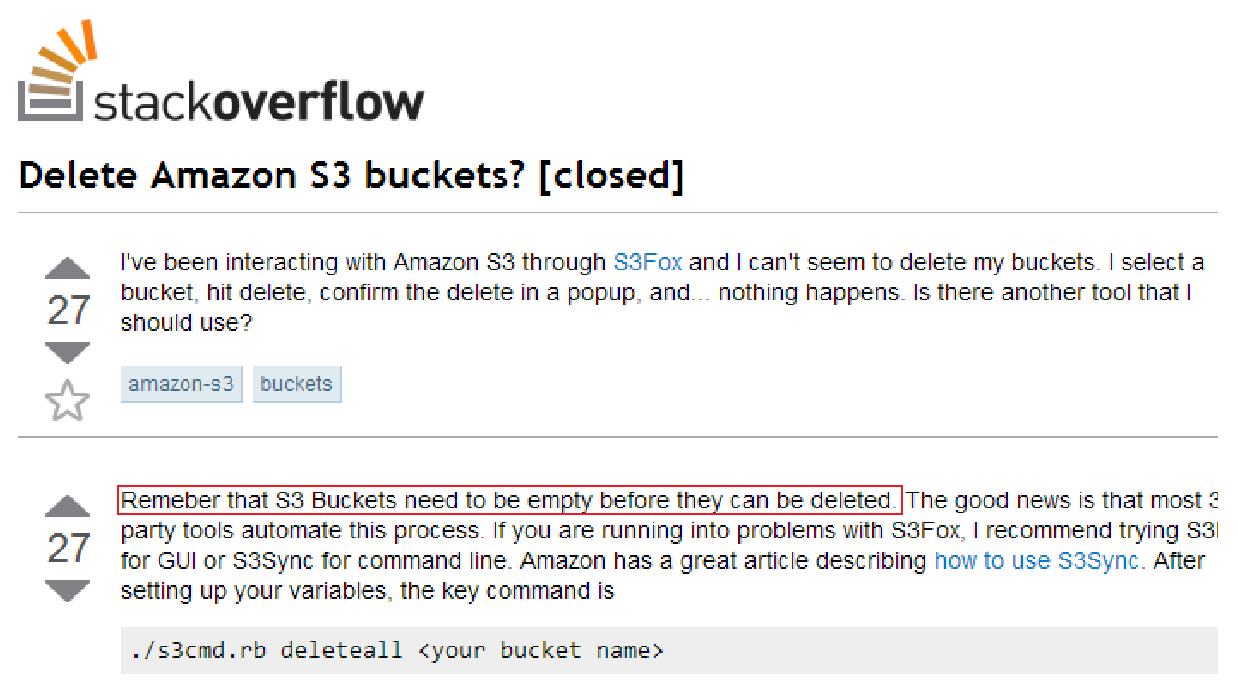
\includegraphics[scale=0.45]{Stackoverflow.eps}
	\end{center}
	\caption{\label{fig:Stackoverflow} The Query posted on Stack Overflow forum regrading Amazon S3 REST API}
\end{figure}

Consider the question asked in \textit{Stack Overflow}~\footnote{{\small \url{http://stackoverflow.com/}}} as shown in Figure~\ref{fig:Stackoverflow}.
Stack Overflow is an online question and answer forum for professional and enthusiast programmers.
The query is about the delete functionality of a third-party software \CodeIn{S3Fox} to interact with \amazonAPI.
The inquisitor complains about an issue in the delete bucket functionality of the \CodeIn{S3Fox}.
The \CodeIn{S3Fox} developers overlooked the constraints in \amazon, causing the issue.
The API document pertaining to the  delete bucket functionality states that before deleting the bucket, the objects in the buckets must be deleted.
\textit{``All objects (including all objects versions and Delete Markers) in the bucket must be deleted before the bucket itself can be deleted''}.
The issue was fixed.
However, one of the forum responses contained a recommendation for the inquisitor to switch to another product.
Customer dissatisfaction, such as was caused by this issue with the delete bucket functionality, can lead to a lose in revenue.
 
The preceding issue can be easily detected using formal analysis tools.
For instance, a specification rule (temporal constraint) can be added to a static checker to verify
the presence of a call to delete object functionality before the call to delete bucket functionality.
%However, existing formal analysis accept only formal specifications but not informal constraints described in natural language.
%Thus, there is need for an approach to automatically translate the constraints described in natural language into a more formal notation.
In next section, we briefly discuss the related work pertinent to our approach.


 









\section{Related work}
\label{sec:related}

% "In contrast" switch up the wording a little bit 

Our proposed approach touches a few research areas such as software verification,
NLP on software engineering artifacts, and document augmentation.
We next discuss the relevant work pertinent to our proposed approach in these areas.

\subsection{Code Contracts - Formal Specifications}
% Define temporal constraints distinction
Design by contracts has been an influential concept in the area of software engineering in the past decade.
A significant amount of work has been done in automated inference of code contracts.
There are existing approaches that statically or dynamically extract code contracts~\cite{csallner08dysy,NimmerE02:ISSTA,Tillmann:2006:DLM:2105385.2105433}. However, a combination of developer written and automatically inferred contracts seems to be the most effective approach~\cite{Polikarpova2009ISSTA,Flanagan:2001:HAA:647540.730008}.
Furthermore, there are existing approaches that infer code-contract-like specifications
(such as behavioral model, algebraic specifications, and exception specifications) either dynamically\cite{Henkel07discoveringdocumentation,Ghezzi:2009:SIB:1555001.1555057,Henkel:2008:DDA:1363102.1363105} or statically~\cite{Flanagan:2001:HAA:647540.730008,Buse:2008:ADI:1390630.1390664} from source code and binaries.
In contrast, the approach presented in this work infers specifications from the natural language text in API documents,
thus complementing these existing approaches when the source code or binaries of the API library is not available.


\subsection{NLP in Software Engineering}

NLP techniques are increasingly applied in the software engineering domain. 
NLP techniques have been shown to be useful in requirements engineering ~\cite{Sinha2009,Sinha2010,Gervasi2005},
usability of API documents~\cite{Dekel2009}, and other areas~\cite{Zhou2008,Little2009,pandita13:WHYPER}.
We next describe the most relevant approaches.


\textit{1. Access Control Policies}: Xiao et al.~\cite{XiaoFSE2012} and Slankas et al.~\cite{johnSlankasPASSAT13} use shallow parsing techniques to infer Access Control Policy (ACP) rules from natural language text in use cases.
The use of shallow parsing techniques works well on natural language texts in use cases, owing to well formed structure of sentences in use case descriptions.
In contrast, often the sentences in API documents are not well formed.
Additionally, these approaches do not deal with programming keywords or identifiers, which are often mixed within the method descriptions in API documents.

\textit{2. Resource Specifications}: Zhong et al.~\cite{zhong09SE} employ NLP and  Machine Learning (ML) techniques to infer resource specifications from API documents.
Their approach uses machine learning to automatically classify such rules.
In contrast, we attempt to parse sentences based on semantic templates and demonstrate that such an approach preforms reasonably well.
Furthermore, the performance of the proposed approach is dependent on the quality of the training sets used for ML.
In contrast, approach presented in this work is independent of such training set and thus can be easily extended to target respective problems addressed by them.
	
\textit{3. Code Comments}: Tan et al.~\cite{TanSOSP07} and Hwei-Tan et al.~\cite{tcomment} applied an NLP and ML  based approach on code comments/ Javadoc comments to detect mismatches between these comments and implementations. They rely on predefined rule templates targeted towards method invocation and lock related comments, thus limiting their scope both in terms of application area as well as language used in the comments. In contrast, approach presented in this report relies on generic natural language based templates thus relaxing the restriction on the style of the language used to describe specifications.
	
\textit{4. API Description}: Most closely related work to the approach presented here is Pandita et al.~\cite{pandita12:inferring} work on inferring parameter constraints from method descriptions in the API documents. In contrast this approach deals with the temporal constraints. The approach presented here is a significant extension to the infrastructure used in the previous work as documented in Section~\ref{sec:approach}.


\subsection{Augmented Documentation}

Another related field has been that of improving the documentation related to an software API~\cite{Dekel2009,tan2011acomment}. We next describe most relevant approaches. Dekel et al.~\cite{Dekel2009}, were the first to create a tool namely eMoose, an Eclipse~\footnote{\url{http://www.eclipse.org/}} based plug-in that allowed developers to create directives (way of marking the specification sentences) in the default API documentation. These directives are highlighted whenever they are displayed in the eclipse environment. Lee et al.~\cite{lee2012towards} improved upon their work by providing a formalism to the directives proposed by Dekel et al.~\cite{Dekel2009}, thus allowing tool based verification. However, a developer has to manually annotate such directives. In contrast, our proposed approach both identifies the sentences pertaining to temporal constraints and infers the temporal constraints automatically. 

In next section, we briefly introduce the NLP techniques used by our approach.




\section{Background}
\label{sec:background}

Natural language is well suited for human communication, but converting natural language into unambiguous specifications that can be processed and understood by computers is difficult.
However, research advances~\cite{Marneffe06LREC,Marneffe08COLING,Klein03,KleinNIPS03} have increased the accuracy of existing NLP techniques to annotate the grammatical structure of a sentence.
These advances in NLP have inspired researchers/ practitioners~\cite{pandita12:inferring, pandita13:WHYPER, johnSlankasPASSAT13, XiaoFSE2012, thummalapentaICSE12} to adapt/apply NLP techniques to solve problems in SE domain.

In particular, this work proposes novel techniques on top of previously proposed techniques~\cite{pandita12:inferring, pandita13:WHYPER} to demonstrate the effectiveness of applying NLP on API documents.
We next briefly introduce the techniques used in this work that have been grouped into broad categories.
We first introduce the core NLP techniques used in this work.
We then introduce the SE specific NLP techniques proposed in previous work~\cite{pandita12:inferring,pandita13:WHYPER} that are used in this work.

\subsection{Core NLP techniques}
\label{sub:CoreNLPback}

%Recently, a lot of exciting work has been carried out in the area of Natural Language Processing (NLP), with existing NLP techniques proving to be fairly accurate in highlighting grammatical structure of a natural language sentence. However, existing NLP techniques are still in the processing phase and not in understanding phase.  We briefly introduce the NLP techniques used in this work.


\textbf{Parts Of Speech (POS) tagging}~\cite{Klein03,KleinNIPS03}. Also known as \textit{`word tagging'}, \textit{`grammatical tagging'} and \textit{`word-sense disambiguation'}, these techniques aim to identify the part of speech (such as noun, verbs, etc.), a particular word in a sentence belongs to. The most commonly used technique is to train a classification parser over a previously known data set. Current state of the art approaches have demonstrated to be effective in classifying POS tags for well written news articles.

\textbf{Phrase and Clause Parsing}. Also known as chunking, this technique divides a sentence into a constituent set of words (or phrases) that logically belong together (such as a Noun Phrase and Verb Phrase). Chunking thus further enhances the syntax of a sentence on top of POS tagging. Current state-of-the-art approaches can effectively classify phrases and clauses over well written news articles.

\textbf{Typed Dependencies}~\cite{Marneffe06LREC,Marneffe08COLING}. The Stanford typed dependencies representation  is designed to provide a simple description of grammatical relationships directed towards non-linguistics experts to perform NLP related tasks. It provides a hierarchical structure for the dependencies with precise definitions of what each dependency represents, thus facilitating machine based manipulation of natural language text.

%\textbf{Named Entity Recognition}~\cite{Finkel05ACL}. Also known as \textit{`entity identification'} and \textit{`entity extraction'}, these techniques are a subtask of information extraction that aims to classify words in a sentence into predefined categories such as names, quantities, expression of times, etc. These techniques help in associating predefined semantic meaning to a word or a group of words (phrase), thus facilitating semantic processing of named entities. 

%\textbf{Co-reference Resolution}~\cite{RaghunathanEMNLP10,LeeCoNLL11}. Also known as \textit{`anaphora resolution'}, these techniques aim to identify multiple expressions present across (or within) the sentences, that point out to the same thing or \textit{`referant'}. These techniques are useful for extracting information; especially if the information encompasses many sentences in a document.


\subsection{SE specific NLP techniques}
\label{sub:SENLPback}

\textbf{Programming keywords}~\cite{pandita12:inferring}. Accurate annotation of POS tags in a sentence is fundamental to effectiveness of any advanced NLP technique.
However, as mentioned previously, POS tagging works satisfactorily on well written news articles which does not necessary entail that the tagging works satisfactorily on domain specific text as well.
Thus, noun boosting is a necessary precursor to application of POS tagging on domain specific text.
In particular, with respect to API documents certain words have a different semantic meaning, in contrast to general linguistics that causes incorrect annotation of POS tags.

Consider the word \CodeIn{POST} for instance. 
The online Oxford dictionary\footnote{\url{http://oxforddictionaries.com/us/definition/american_english/post?q=POST}} has eight different definition of word \CodeIn{POST}, and none of them describes \CodeIn{POST} as an HTTP method\footnote{In HTTP vocabulary \CodeIn{POST} means: \textit{``Creates a new entry in the collection.
The new entry's URI is assigned automatically and is usually returned by the operation''}}
supported by REST API.
Thus existing POS tagging techniques fail to accurately annotate the POS tags of the sentences involving word \CodeIn{POST}.  

Noun Boosting identifies such words from the sentences based on a domain-specific dictionaries, and annotates them appropriately.
The annotation assists the POS tagger to accurately annotate the POS tags of the words thus in turn increasing accuracy of advanced NLP techniques such as chunking and typed dependency annotation.

\textbf{Lexical Token Reduction}~\cite{pandita13:WHYPER}.
These are a group of generic preprocessing heuristics to further improve the accuracy of core NLP techniques.
The accuracy of core NLP techniques is inversely proportional to the number of lexical tokens in a sentence.
Thus, the reduction in the number of lexical tokens greatly increases the accuracy of core NLP techniques. 
In particular, following heuristics have been used in previous work to achieve the desired reduction of lexical tokens:

\begin{itemize}

\item \textbf{Period Handling}. Besides marking the end of a sentence in simplistic English, the character period (`.') has other legal usages as well such as decimal representation (periods between numbers).
Although legal, such usage hinder detection of sentence boundaries, thus causing core NLP techniques to return incorrect or imprecise results.
The text is pre-processed by annotating these usages for accurate detection of sentence boundaries.
	
\item \textbf{Named Entity Handling}. Sometimes a sequence of words correspond to the name of entities that have a specific meaning collectively.
For instance, consider the phrases \textit{``Amazon S3'', ``Amazon simple storage service''}, which are the names of the service.
Further resolution of these phrases using grammatical syntax is unnecessary and would not bring forth any semantic value.
Also these phrases contribute to length of a sentence that in turn negatively affects the accuracy of core NLP techniques.
This heuristic annotates the phrase representing the name of the entities as a single lexical token.
	
\item \textbf{Abbreviation Handling}. Natural-language sentences often consist of abbreviations mixed with text.
This phenomenon can result in subsequent components to incorrectly parse a sentence.
This heuristic finds such instances and annotates them as a single lexical unit.
For example, text followed by abbreviations such as \textit{``Access Control Lists (ACL)''} is treated as single lexical unit.
Detecting such abbreviations is achieved by using the common structure of abbreviations and encoding such structures into regular expressions.
Typically, regular expressions provide a reasonable approximation for handling abbreviations.  

\end{itemize}

\textbf{Intermediate-Representation Generation}~\cite{pandita13:WHYPER}.
This technique accepts the syntax-annotated sentences and builds a First-Order-Logic(FOL) representation of the sentence.
Earlier researches have shown the adequacy using FOL for NLP related analysis tasks~\cite{Sinha2009,Sinha2010,pandita12:inferring}.
In particular, WHYPER~\cite{pandita13:WHYPER} demonstrates the effectiveness of this technique, by constructing an intermediate representation generator based on shallow parsing~\cite{Branimir2000} techniques. 
The shallow parser itself is implemented as a sequence of cascading finite state machines based on the function of Stanford-typed dependencies~\cite{Marneffe06LREC,Marneffe08COLING,Klein03,KleinNIPS03}.


In next section we describe our generic approach to infer temporal constraints from API documents. 
\section{Approach Overview}
\label{sec:approach}
%\vspace{-2mm}

\begin{figure}
	\centering
		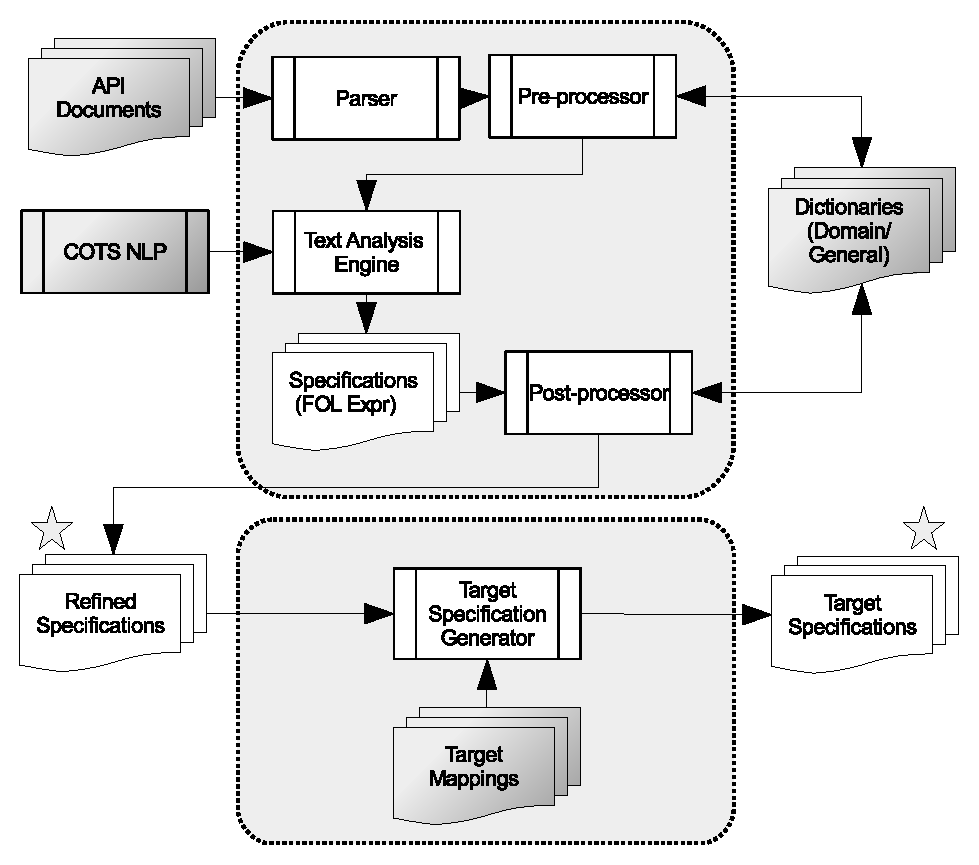
\includegraphics[scale=0.45]{approach.eps}
	\caption{Overview of \tool\ approach}
	\label{fig:approachOverview}
\end{figure}

We next present our approach for inferring specifications from the method descriptions in API Documents.
Figure~\ref{fig:approachOverview} gives an overview of our approach.
Our approach consists of five major components: a preprocessor, a text-analysis engine, a semantic graph generator, specification extractor, and a type analyzer.

The preprocessor accepts API documents and preprocesses the sentences in the method description, such as annotating sentence boundaries and reducing lexical tokens.
The text-analysis engine accepts the pre-processed sentences and annotates them using an NLP parser.
The text-analysis engine further transforms the annotated sentences into the first-order-logic (FOL) representation. The semantic graph generator accepts the API documents and generates the semantic graphs that are leveraged by specification extractor component.
The type analyzer component infers temporal constraints encoded in the type system of a language by analyzing the API methods parameter and return types.
Finally, the specification extractor then leverages the semantic graphs to infer temporal constraints from the FOL representation of a sentence.
We next describe each component in detail.


\subsection{Preprocessor}
\label{sub:prep}

The preprocessor accepts the API documents and first extracts method descriptions from it.
In particular, the preprocessor extracts the following fields within method descriptions: 
1) \textit{Summary of the API method},
2) \textit{Summary and type information of parameters of the API method}, 
3) \textit{Summary and type information of return values of the method}, and
4) \textit{Summary and type information of exceptions thrown by the methods}.

This step is required to extract the desired descriptive text from the various presentation styles of the API documents.
In particular, different API documents may have different styles of presenting information to developers.
This difference in style may include the difference in the level of detail presented to the developer.
Our approach thus relies on only basic fields that are trivially available for API methods across different presentation styles. 

After extracting desired information, the natural language text is further preprocessed to be analyzed by subsequent components.
The preprocessing steps are required to increase the accuracy of core NLP techniques (described in Section~\ref{sub:CoreNLPback}) that are used in the subsequent phases of \tool\ approach.
In particular, the preprocessor first employs the noun boosting followed by heuristics listed under lexical token reduction, as introduced in Section~\ref{sub:SENLPback}.

Although the previous techniques and heuristics significantly lower the number of lexical tokens in a sentence, some sentences may still contain a considerable number of lexical tokens to overwhelm the POS tagger.
To address this issue, we propose a novel technique (\textit{`Frequent Phrases Reduction'}) to further reduce the number of lexical tokens in a sentence by annotating frequent phrases as a single lexical unit.

In particular, we use n-gram based approach as means to achieve this reduction. 
In the fields of computational linguistics and probability, an n-gram is a contiguous sequence of n words from a given sequence of text or speech. 
We first calculate the most frequently occurring n-grams in the text body. 
In particular, we are interested in the n-grams of length 4 or greater to achieve a reasonable reduction. 
We then prune the list of n-grams based on a subsumption. 
We consider a n-gram of length k ($n_k$) to subsume n-gram of length k-1 ($n_{k-1}$) iff $n_{k-1}$ is a substring of ($n_k$) and the frequency of occurrence of $n_{k-1}$ equals frequency of occurrence of $n_{k}$.
Finally, we rank the list of n-grams based on the frequency of their occurrence in the text, and select top-k n-grams for reduction.
For instance, \textit{Amazon Simple Storage Service}, \textit{an I/O Error Occurs}, and \textit{end of stream} are the examples of such n-grams detected by our approach.
%\begin{figure}[t]
%\begin{CodeOut}
%\begin{alltt}
%01: 
%04:
%\end{alltt}
%\end{CodeOut}\vspace*{-2ex}
%\caption{\label{fig:methodAPI} The method description of the \CodeIn{DefineObjectProperty} method in Facebook API}\vspace*{-4ex}
%\end{figure}
\\
\textbf{Prototype Implementation.}
Currently our prototype implementation works with online \amazon\ and JDK API. 
However, almost all of the developer documents are provided online as structured webpages.
Thus, current implementation of preprocessor can be easily extended to extract the desired information from any API developer documents.    

Additionally, in current implementation we have manually built the domain dictionaries for preprocessing using the glossary of terms collected from the websites pertaining to REST and Java API.
We further leveraged the HTML style information in \amazon\ to look for words that were highlighted in code like format. We further leveraged WordNet to maintain a static lookup table of shorthand words to aid named entity handling and abbreviation handling. 

 
Finally, to achieve  n-gram reduction we used Apache Lucene$^{\textregistered}$~\cite{lucene}.
Apache Lucene is a high-performance, full-featured text search engine library written entirely in Java.
It is a technology suitable for nearly any application that requires full-text search, especially cross-platform.

%Although a POS tagger can be retrained to achieve these pre-processing steps, we prefer annotations to make our approach independent of any specific NLP infrastructure, thus ensuring interoperability with various POS taggers.
	
\subsection{NLP Parser}


The NLP parser accepts the pre-processed documents and annotates every sentence within each document using core NLP techniques described in Section~\ref{sub:CoreNLPback}.
From an implementation perspective, we chose the Stanford parser~\cite{Manning:01}.
However, this component can be implemented using any other existing NLP libraries or approaches.
In particular, we annotate each sentence with POS tags, named-entity annotations and Stanford-typed dependencies.
For more details on these techniques and their application, please refer to ~\cite{Marneffe06LREC, Marneffe08COLING, pandita12:inferring, pandita13:WHYPER, thummalapentaICSE12}.

%\begin{figure}
%	\centering
%%		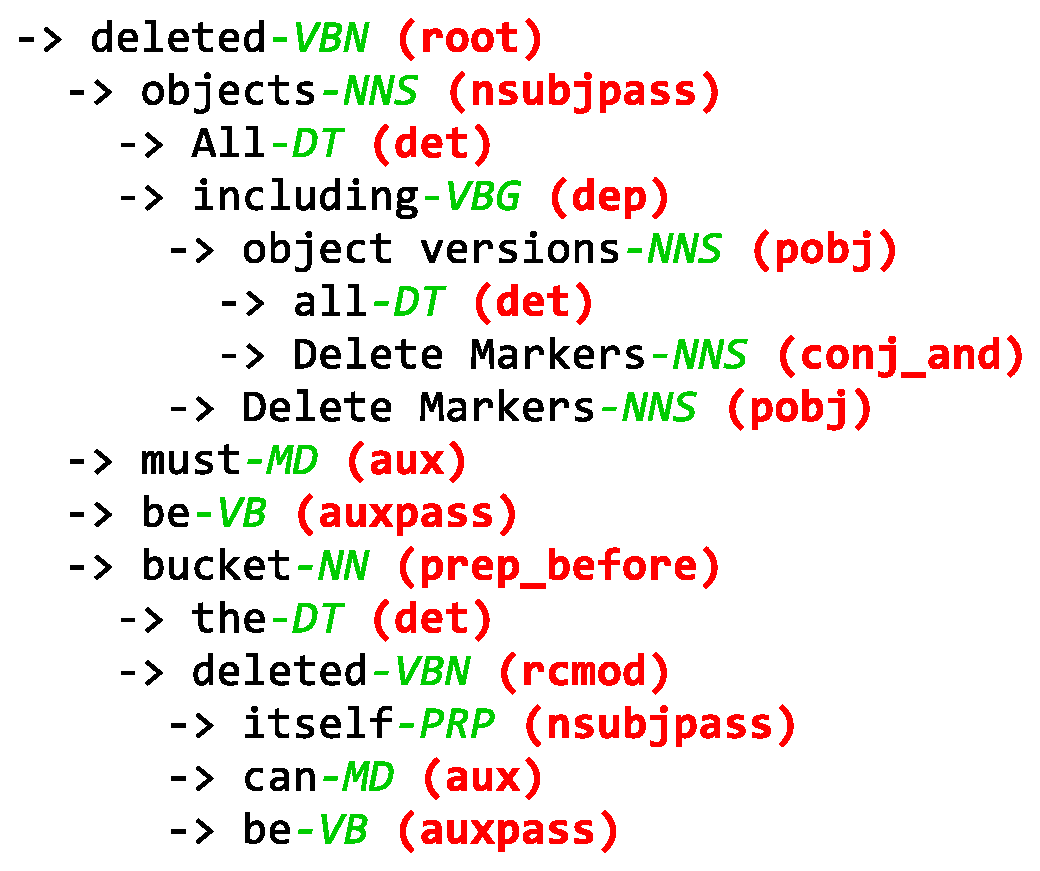
\includegraphics[scale=0.6]{StanfordAnnotated.eps}
%	\caption{Sentence annotated with Stanford dependencies}
%	\label{fig:standep}
%\end{figure}
%
%Next we use an example to illustrate the annotations added by the NLP Parser. Consider the example sentence \textbf{\textit{``Also you can share the yoga exercise to your friends via Email and SMS.''}}, that indirectly refers to the READ\_CONTACTS permission. Figure~\ref{fig:standep} shows the sentence annotated with Stanford-typed dependencies. The words in red are the names of dependencies connecting the actual words of the sentence (in black). Each word is followed by the Part-Of-Speech (POS) tag of the word (in green). For more details on Stanford-typed dependencies and POS tags, please refer to ~\cite{Marneffe06LREC,Marneffe08COLING}.

\subsection{Text Analysis Engine}
\label{sub:TAE}
%
%\begin{figure}
%	\centering
%	%	\includegraphics[scale=0.65]{taeRep.eps}
%	\caption{First-order logic representation of annotated sentence in Figure~\ref{fig:standep}}
%	\label{fig:FOLRep}
%\end{figure}

The text analysis engine component accepts the annotated documents and creates an intermediate representation of each sentence.
We define our representation as a tree structure that is essentially a FOL expression.
Research literature provides evidence of the adequacy of using FOL for NLP related analysis tasks~\cite{Sinha2009,Sinha2010,pandita12:inferring, pandita13:WHYPER}.

In our representation, every node in the tree except for the leaf nodes is a predicate node. 
The leaf nodes represent the entities.
The children of the predicate nodes are the participating entities in the relationship represented by the predicate.
The first or the only child of a predicate node is the governing entity and the second child is the dependent entity.
Together the governing entity, predicate and the dependent entity node form a tuple.  


As described in Section~\ref{sub:SENLPback} the intermediate representation generation technique is based on the principle of shallow parsing~\cite{Branimir2000}. 
In particular, the intermediate-representation technique is implemented as a function of Stanford-typed dependencies~\cite{Marneffe06LREC,Marneffe08COLING,KleinNIPS03}, to leverage the semantic information encoded in Stanford-typed dependencies.


However, we observed that such implementation is overwhelmed by complex sentences.
This limitation mandates the use of additional novel technique of \textit{`Frequent Phrases Reduction'} in preprocessing phase.
We further improve the accuracy of intermediate-representation generation by proposing a hybrid approach, i.e. taking into consideration both the POS tags as well as Stanford-typed dependencies.
The POS tags which annotate the syntactical structure of a sentence are used to further simplify the constituent elements in a sentence. 
We then use the Stanford-typed dependencies that annotate the grammatical relationships between words to construct our FOL representation.
Thus, the intermediate representation generator used in this work is a two phase process as opposed to previous work~\cite{pandita12:inferring, pandita13:WHYPER}. 
We next describe these two phases:

\textbf{POS Tags}: We first parse a sentence based on the function of POS tags. 
In particular, we use semantic templates to logically break a sentences into smaller constituent sentences. 
For instance, consider the sentence:

\begin{center}
\scriptsize``All objects (including all object versions and Delete Markers) in the bucket must be deleted before the bucket itself can be deleted.''. \normalsize
\end{center}

The Stanford parser inaccurately annotates the Stanford-typed dependencies of the sentence because of presence of different clauses acting on different subject-object pairs.
We thus break down the sentence into two smaller tractable sentences:

\begin{center}
\scriptsize \textit{``All objects in the bucket must be deleted before the bucket itself can be deleted.}''
	
\textit{``All objects including all object versions and Delete Markers.''}\normalsize 
\end{center} 


Table~\ref{tab:semanticTemplates} shows a list the semantic templates used in this phase.
Column ``Template'' describes conditions where the template is applicable and Column ``Summary'' describes the action taken by our shallow parser when the template is applicable.
All of these semantic templates are publicly available on our project website\footnote{\url{https://sites.google.com/site/temporalspec}}.
With respect to the previous example the template 3 \textit{( A noun phrase followed by another noun/pronoun/verb phrase in brackets)} is applicable.
Thus our shallow parser breaks the sentence into two individual sentences.
	 
\begin{table*}
\begin{center}

\caption{Semantic Templates}
    \begin{tabular}{  l  p{5cm} p{10cm} }
    \topline
    \headcol  \textbf{S No.} 	& \textbf{Template} & \textbf{Summary} \\
    \midline
    
    1. 		& Two sentences joined by a conjunction & Sentence is broken down into two individual sentences with the conjunction term serving as the connector between two. \\
\rowcol    2. 		& Two sentences joined by a ``,''& Sentence is broken down to individual independent sentences \\
    3.		& A noun phrase followed by another noun/pronoun/verb phrase in brackets & Two individual sentences are formed. The first sentence is  the same as the parent sentence sans the noun/pronoun.verb phrase in bracket. The second sentence constitutes of the noun phrase followed by  noun/pronoun/verb phrase without the brackets.\\
\rowcol    4.		& A noun phrase by a conditional phrase in brackets & Two individual sentences are formed. The first sentence is the same as the parent sentence sans the conditional phrase in bracket. The second sentence constitutes of noun phrases followed by conditional in the bracket.\\ 
    5.		& A conditional phrase followed by a sentence & Two dependent sentences are formed. The first sentence constitutes the conditional phrase. The second sentence constitutes rest of the sentence.\\
\rowcol    6.		& A sentence in which the parent verb phrase is over two child verb phrases joined by a conjunction & Two dependent sentences are formed where the dependency is the conjunction. The first sentence is formulated by removing conjunction and second child verb phrase. The second sentence is formulated by removing conjunction and first child verb phrase. \\ 
\bottomlinec
    \end{tabular}
	\label{tab:semanticTemplates}
\end{center}
\end{table*}

\textbf{Stanford-typed Dependencies}: This phase is equivalent to the intermediate-representation technique described in Section~\ref{sub:SENLPback}.

\subsection{Specification Extractor}
\label{sub:SE}

This component accepts the FOL representation of the sentence from the previous component,
then extracts the temporal constraints if present in a sentence. 
Specification Extractor then classifies the sentence as a specification 
sentence (containing temporal constraint) candidate based on following ordered set of rules:

\begin{enumerate}
	\item The sentence is not from parameter summary or return variable summary.
	Typically such sentences describe pre-post conditions as opposed to temporal constraints this approach addresses.
	\item The sentences contains modal modifiers such as ``\textit{can, could, may, must, should}'' expressing necessity.
	Typically, presence of such modal modifier is a strong indicator of presence of constraints imposed by an API developer
	\item If the sentence does not contain modal modifiers described previously, sentence must contain temporal modifier relationship, identified by Stanford-typed dependency parser.
	Typically, presence of temporal modifier is an indicator of presence of temporal information.  
	\item If rules 2 and 3 don't apply then the sentences should be a conditional sentence, identified by the presence of keywords such as ``\textit{if}''.
\end{enumerate} 

Once a candidate sentence is identified, this component selects an semantic graph.
In particular, the semantic graph of the API class to which the candidate sentence belongs to selected.
A semantic graph constitutes the keyword representation of the classes and the corresponding applicable actions. 
Figure~\ref{fig:knowledge} shows a sub-graph of  graph for \CodeIn{BufferedInputReader} class.
The phrases in solid rectangles are synonyms of the class name \CodeIn{BufferedInputReader}.
The phrases in rounded rectangle are the actions applicable on \CodeIn{BufferedInputReader} class.
Section~\ref{sub:ACA} further describes how these graphs are generated.

 
Specification extractor then uses the semantic graph to determine
if a candidate sentence is a specification sentence and if so extract
the action that should be performed prior to the method the sentence
belongs to. Algorithm~\ref{alg:SenAnnotaator} describes this action extraction
process.  

\algsetup{indent=1em}
\begin{algorithm}[t!]
\begin{algorithmic}[1]
\begin{scriptsize}
\REQUIRE K\_Graph $g$, FOL\_rep $rep$ 
\ENSURE String $action$
\STATE $String\ action\ =\ \phi$
\STATE $List\ r\_name\_list\ =\ g.resource\_Names$
\STATE $FOL\_rep\ r'\ =\ rep.findLeafContaining(r\_nam\_list)$
\STATE $List\ actionList\ =\ g.actionList$
\WHILE{$(r'.hasParent)$}
	\IF{$actionList.contains(r'.parent.predicate)$}
		\STATE $action\ =\ actionList.matching(r'.parent.predicate)$
		\STATE $break$
	\ELSE
		\IF{$actionList.contains(r'.leftSibling.predicate)$}
			\STATE $action\ =\ actionList.matching(r'.leftSibling.predicate)$
			\STATE $break$
		\ENDIF
	\ENDIF
	\STATE $r'\ =\ r'.parent$
\ENDWHILE
\RETURN $action$
\end{scriptsize}
\end{algorithmic}
\caption{Action\_Extractor}
\label{alg:SenAnnotaator}
\end{algorithm} 

Our algorithm systematically explores the FOL representation
of the candidate sentence to determine if a sentence
describes a temporal specification. First, our algorithm
attempts to locate the occurrence of class name or its synonym
within the leaf nodes of the FOL
representation of the sentence (Line 3). The method
findLeafContaining(r\_name\_list) explores the FOL representation
to find a leaf node that contains either the class name
or one of its synonyms.
In particular, we use WordNet~\cite{wordnet} and Lemmatisation
to deal with synonyms of a word in question to find appropriate
matches. Once a leaf node is found, we systematically
traverse the tree from the leaf node to the root,
matching all parent predicates as well as immediate child
predicates [Lines 5-16].

Our algorithm matches each of the traversed predicate
with the actions associated with the class defined in
semantic graph. Similar to matching entities, we also
employ WordNet and Lemmatisation to deal with
synonyms to find appropriate matches. If a match is
found, then the matching action name is returned.

\subsection{Semantic-Graph Generator}
\label{sub:ACA}

A key way of identifying reference to a method within the API in our proposed approach is the employment of a semantic graph of an API.
In particular, we propose to initially infer such graphs from API documents.
Manually creating a semantic graph is prohibitively time consuming and may be error prone.
We thus employ a systematic methodology (proposed previously in ~\cite{pandita13:WHYPER}) to infer such semantic graphs from API documents that can potentially be automated.
We first consider the name of the class for the API document in question.
We then find the synonyms terms used refer to the class in question.
The synonym terms are listed as by breaking down the camel-case notation in the class name.
This list is further augmented by listing the name of the parent classes and implemented interfaces if any. 

\begin{figure}
	\centering
		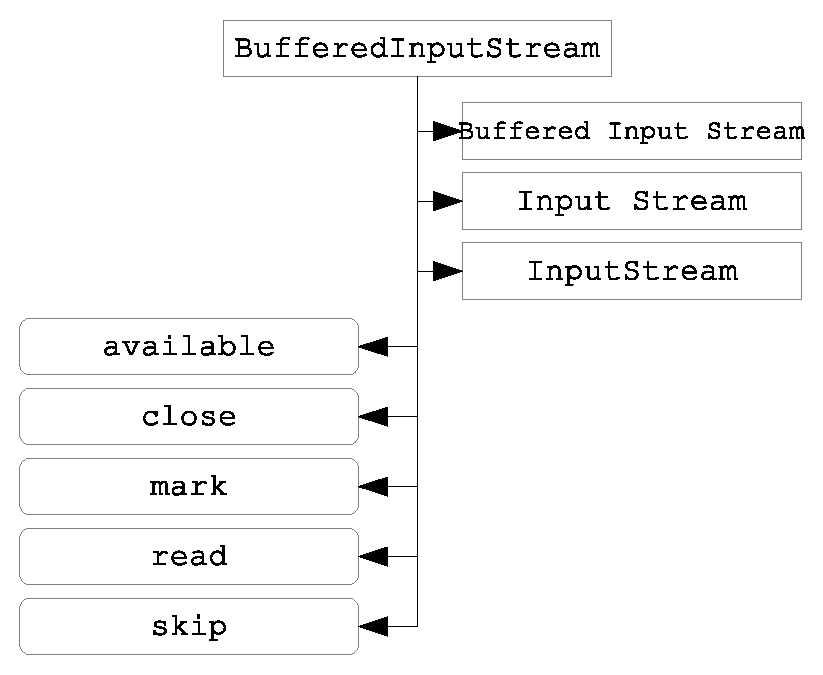
\includegraphics[scale=0.4]{KnowledgeGraph.eps}
	\caption{Semantic Graph for the \CodeIn{BufferedInputStream} class in Java}
	\label{fig:knowledge}
\end{figure} 


We then systematically inspect the member methods to identify actions applicable to the objects represented by the class. From the name of a public method (describing a possible action on the object), we extract verb phrases. The verb phrases are used as the associated actions applicable on the object. For instance, \CodeIn{BufferedInputReader} defines operations available, close, mark, and so on. We associate these operations with the objects of type \CodeIn{BufferedInputReader}. Figure~\ref{fig:knowledge} shows a sub-graph of  graph for \CodeIn{BufferedInputReader} class. The phrases in solid rectangles are synonyms of the class name \CodeIn{BufferedInputReader}. The phrases in rounded rectangle are the actions applicable on \CodeIn{BufferedInputReader} class.
  

\subsection{Type Analysis}

As mentioned earlier that some temporal constraints are enforced by the type system in typed Languages.
For instances a method ($m$) accepting input parameter ($i$) of type ($t$) mandates that (at least one) method ($m'$) be invoked whose return value is of type ($t$). To extend the temporal constraints inferred by the analyzing the natural language text, this component infers additional constraints that are encoded
in the type system. Algorithm~\ref{alg:TypeAnalysis} lists the steps followed to infer type based temporal constraints.

The algorithm accepts the list of methods as an input produces a graph with
the nodes representing methods in an API and the directed edges representing temporal constraints.
First, a index is created based on the return types of the method (Line 2).
Second, all methods in an API are added to an unconnected graph (Line 3-4).
Then, for every public method in the input list, the algorithm checks the types
of the input parameters and constructs and directed edge from all the methods whose return value
have the same type to the method in question (Line 14- 20).
The algorithm does not take into consideration the basic parameter types such as integer, string (Line 15).
Additionally, an edge is created from the constructors of a class to the non static members methods of a class (Line 8 -13).
The resultant graph is then returned by the algorithm.


The temporal constraints based on the type information can be extracted by querying the graph. 
The incoming edges to a node denoting a method represents the set of pre-requisite methods.
The temporal constraint being, at least one of the pre-requisite methods must be invoked before invoking the method in question.


\begin{algorithm}[t!]
\begin{algorithmic}[1]
\begin{scriptsize}
\REQUIRE List $methodList$ 
\ENSURE Graph $seq\_Graph$
\STATE $Graph\ seq\_Graph\ =\ \phi$
\STATE $Map\ idx\ = createIdx(methodList)$

\FORALL{$Method\ mtd\ in\ methodList$} 
	\STATE $seq\_Graph.addVertex(mtd)$
\ENDFOR

\FORALL{$Method\ mtd\ in\ methodList$} 
	\IF{$mtd.isPublic()$}
		\IF{$!mtd.isStatic()$}
			\STATE $List\ preList\ =\ idx.query(mtd.declaringType)$
			\FORALL{$Method\ mtd'\ in\ preList$}
				\STATE $seq\_Graph.addEdge(mtd',mtd)$
			\ENDFOR
		\ENDIF
		\FORALL{$Parameter\ param\ in\ mtd.getParameters()$}
			\IF{$!isBasicType(param.Type)$}
				\STATE $List\ preList\ =\ idx.query(paramType)$
				\FORALL{$Method\ mtd'\ in\ preList$}
					\STATE $seq\_Graph.addEdge(mtd',mtd)$
				\ENDFOR				
			\ENDIF
		\ENDFOR
	\ENDIF
\ENDFOR
\RETURN $seq\_Graph$
\end{scriptsize}
\end{algorithmic}
\caption{Type\_Sequence\_Builder}
\label{alg:TypeAnalysis}
\end{algorithm} 


\section{Evaluation}
\label{sec:evaluation}

We next present the evaluation we conducted to assess the effectiveness of \tool. In our evaluation, we address three main research questions:

\begin{itemize}
	\item\textbf{RQ1}: What are the precision and recall of \tool\ in identifying temporal constraints from sentences written in natural language?
	Answer to this question quantifies the effectiveness of \tool\ in identifying constraint sentences.
	\item\textbf{RQ2}: What is the accuracy of \tool\ in inferring temporal constraints from constraint sentences in the API documents?
	Answer to this question quantifies the effectiveness of \tool\ in inferring temporal constraints from constraint sentences. 
	\item\textbf{RQ3}: What is the degree of the overlap between the temporal constraints inferred from natural language text in comparison to the typed-enforced temporal constraints?
	
 
\end{itemize}

\subsection{Subjects}
\label{sub:subject}

We used the API documents of the following two libraries as subjects for our evaluation. 
\begin{itemize}
	\item \amazonAPI\: provides a REST based web services interface to store and retrieve data on the web.
	Furthermore, \CodeIn{Amazon S3} also empowers a developer with rich set of API methods to access a highly scalable, reliable, secure, fast, and inexpensive infrastructure. 
	\CodeIn{Amazon S3} is reported to store more than 2 trillion objects as of April 2013 and gets over 1.1 million requests per second at peak time~\cite{amazons3stats}.
	
	\item \paypalAPI\: provides a REST based web service interface to facilitate online payments and money transfer.
	\CodeIn{PayPal} reports to have handled \$56.6 billion(USD) worth of transactions (total value of transactions) in just the third quarter of 2014. 
	
	\item\CodeIn{java.io} : is one of a popular packages in \CodeIn{Java} programming language. The package provides APIs for system input and output through data streams, serialization and the file system, which are one of the fundamental functionalities provided by a programming language.
\end{itemize}
We chose \CodeIn{Amazon S3}, \CodeIn(PayPal) and \CodeIn{java.io} APIs as our subjects because they are popular and contain decent documentation.

\subsection{Evaluation Setup} 
We first manually annotated the sentences in the API documents of the two APIs.
Two authors manually labeled each sentence in the API documentation as sentence containing 
temporal constraints or not.
We used \CodeIn{cohen kappa}~\cite{carletta1996assessing} score to statistically measure
the inter-rater agreement.
The \CodeIn{cohen kappa} score of the two authors was .66 (on a scale of 0 to 1), 
which denotes a statically significant agreement~\cite{carletta1996assessing}. 
After the authors classified all the sentences, they 
discussed with each other to reach a consensus on the sentences they classified differently. 
We use these classified sentences as the golden set for calculating precision and recall.

To answer RQ1, we measure the number of true positives ($TP$), false positives ($FP$), true negative ($TN$), and false negatives ($FN$)
in identifying the constraint sentences by \tool.
We define constraint sentence as a sentence describing a temporal constraints.
We define the $TP$, $FP$, $TN$, and $FN$ of \tool\ as follows:

\begin{enumerate}
	\item $TP$: A sentence correctly identified by \tool\ as constraint sentence.
	\item $FP$: A sentence incorrectly identified by \tool\ as constraint sentence.
	\item $TN$: A sentence correctly identified by \tool\ as not a constraint sentence.
	\item $FN$: A sentence incorrectly identified by \tool\ as not a constraint sentence.
\end{enumerate}


In statistical classification~\cite{Olson08}, \CodeIn{precision} is defined as a ratio of
number of true positives to the total number of items reported to be true,
\CodeIn{recall} is defined as a ratio of number of true positives to the total number
of items that are true. \CodeIn{F-Score} is defined as the weighted harmonic mean of 
\CodeIn{precision} and \CodeIn{recall}. Higher value of \CodeIn{precision}, \CodeIn{recall}, and \CodeIn{F-Score}
are indicative of higher quality of the constraint statements inferred using 
\tool. based on the calculation of $TP$, $FP$, $TN$, and $FN$ of \tool\ defined
previously we computed the \CodeIn{precision}, \CodeIn{recall}, and \CodeIn{F-Score} of \tool\ as follows:


\begin{center}

$Precision$ = $\frac{TP}{TP + FP}$

$Recall$ = $\frac{TP}{TP + FN}$

$F-Score$ = $\frac{2 X Precison X Recall}{Precision + Recall}$
\end{center}


To answer RQ2, we manually verified the temporal constraints inferred from constraint sentences by \tool.
However, we excluded the type-enforced temporal constraints inferred using Algorithm~\ref{alg:TypeAnalysis}, described in Section~\ref{sec:approach}.
We excluded the type-enforced constraints because they are correct by construction and are by default enforced by modern IDE's such as eclipse. 
We then measure $accuracy$ of \tool\ as the ratio of the total number of temporal constraints that
are correctly inferred by \tool\ to the total number of constraint sentences. Two authors
independently verified the correctness of the temporal constraints inferred by \tool.
We define the \CodeIn{accuracy} of \tool\ as the ratio of constraint sentences with correctly inferred temporal constraints
to the total number of constraint sentences. 
Higher value of \CodeIn{accuracy} is indicative of effectiveness of \tool\ in inferring temporal constraints from constraint sentences.


To answer RQ3, we counted the overlap in the temporal constraints inferred by \tool\ 
from the natural language text in API documents to the type-enforced temporal constraints
inferred using Algorithm~\ref{alg:TypeAnalysis}, described in Section~\ref{sec:approach}.

\subsection{Results}

We next present our evaluation results.

\begin{table*}
\begin{center}

\caption{Evaluation Results (Identification)}

\begin{tabular}{rlccccccccc}
\topline
\headcol S. No. & Trainer	& P$_{wrd}$	& R$_{wrd}$	& F$_{wrd}$	& P$_{ftr}$	& R$_{ftr}$	& F$_{ftr}$	& P$_{\Delta}$	& R$_{\Delta}$	& F$_{\Delta}$	\\
\midline 
		 1 		& 				& 662 	& 2417 		& 78 		& 88 		& 57 		& 31 		& 21 			& 64.8 			& 73.1 			\\ 
\rowcol  2		& \amazonAPI 	& 662 	& 2417 		& 78 		& 88 		& 57 		& 31 		& 21 			& 64.8 			& 73.1 			\\ 
		 3		& \paypalAPI 	& 662 	& 2417 		& 78 		& 88 		& 57 		& 31 		& 21 			& 64.8 			& 73.1 			\\ 
\rowcol 		& Average 		& 662 	& 2417 		& 78 		& 88 		& 57 		& 31 		& 21 			& 64.8 			& 73.1 			\\ 
\bottomlinec
%----------------- END TABLE DATA ------------------------ 
\multicolumn{11}{p{6.5in}}{\small
All values are average over 10-fold cross validation;
P: Precision; R: Recall; F: F-Score;
$_{wrd}$: No features used for training;
$_{ftr}$: features used for training;
$_{\Delta}$: improvement factor ($_{ftr}$ - $_{wrd}$)} \\ 
\end{tabular}
\label{tab:results}
\end{center}
\end{table*}


\begin{table}
\begin{center}

\caption{Evaluation Results (Inference)}

\begin{tabular}{lccccc}
\topline
\headcol 	API 		& Mtds 	& Sen 	& Sen$_C$ 	& Spec$_{ICON}$ 	& Acc(\%)\\
\midline 
			java.io 	& 662 	& 2417 	& 78 		& 56 				& 71.8\\ 
\rowcol 	Amazon S3 REST 	& 51 	& 1492 	& 12		& 7 				& 58.3\\ 
			Paypal REST 	& 33	& 151 	& 20 		& 					& \\ 
\rowcol 	Total 		& 746 	& 4060 	& 90		& 63 				& 70.0$^*$\\ 
\bottomlinec
%----------------- END TABLE DATA ------------------------ 
\multicolumn{6}{p{3.25in}}{\small
$^*$ Average;
Mtds: Total no. of Methods; Sen: Total no. of Sentences; Sen$_C$: Total no. of constraint Sentences; Acc: Accuracy
Spec$_{ICON}$: Total no. of temporal constraint correctly identified by \tool;
} \\ 
\end{tabular}
\label{tab:results}
\end{center}
\end{table}


\subsubsection{RQ1: Effectiveness in Identifying Constraint Sentences}


In this section, we quantify the effectiveness of \tool\ in identifying constraint sentences by answering RQ1.
Table~\ref{tab:results} shows the effectiveness of \tool\ in identifying constraint sentences.
Column ``API'' lists the names of the subject API. 
Columns ``Mtds'' and ``Sen'' lists the number of methods and sentences in each subject API's.
Column ``Sen$_C$'' list the number of manually identified constraint sentences.
Column ``Sen$_{ICON}$'' lists the number of sentences identified by \tool\ as constraint sentences. 
Columns ``TP'', ``FP'', ``TN'', and ``FN'' represent the number of \CodeIn{true positives}, \CodeIn{false positives}, \CodeIn{true negatives}, and \CodeIn{false negatives}, respectively. 
Columns ``P(\%)'', ``R(\%)'', and ``F$_S$(\%)'' list percentage values of \CodeIn{precision}, \CodeIn{recall}, and \CodeIn{F-score} respectively. 
Our results show that, out of 3,909 sentences, \tool\ effectively identifies constraint sentences with the average \CodeIn{precision}, \CodeIn{recall}, and \CodeIn{F-score} of 65.0\%, 72.2\%, and 68.4\%, respectively.

 

%We next present an example to illustrate how \tool\ incorrectly identifies a sentence as a constraint sentence. \textbf{A example goes here}
We next present an example to illustrate how \tool\ incorrectly identifies a sentence as a constraint sentence (producing false positives).
For instance, consider the sentence ``\textit{This is done by flushing the stream and then closing the underlying output stream.}'' from  \CodeIn{close} method description from \CodeIn{PrintStream} class.
\tool\ incorrectly identifies the action ``flush'' being performed before the action ``close''.
However \tool\ fails to make the distinction that it happens internally (enforced in the body) in the method.
\tool, thus incorrectly identifies the sentence as a constraint sentence.   


Another major source of FPs is the incorrect parsing of sentences by the underlying NLP infrastructure
and/or inadequacy of generic dictionaries for synonym analysis.
For instance, consider the sentence ``\textit{If this stream has an associated channel then the channel is closed as well.}''
from the \CodeIn{close} method description from \CodeIn{FileOutputStream}.
The sentence describes an effect that happens as a result of calling the \CodeIn{close} method and does not describe any temporal constraint.
However, \tool\ annotates the sentence as a constraint sentence because underlying Wordnet dictionaries matches the word ``has'' as a synonym of ``get''.
This incorrect matching in turn causes \tool\ to incorrectly annotate the sentence as constraint sentence
because ``has'' is matched against \CodeIn(get) method in \CodeIn{FileOutputStream}.
We observed 8 instances of previously described example in our results.

If we manually fixed the Wordnet dictionaries to not match ``has'' and ``get'' as synonyms,
our precision is further increased to 70.8\% effectively increasing the F-Score of \tool\ to 71.2\%.
Although an easy fix, we refrained from including such modifications for reporting the results to stay true to our approach.
In the future, we plan to investigate techniques to construct better domain dictionaries for software API. 

We next present an example to illustrate how \tool\ fails identify a constraint sentence (producing false negative).
False negatives are undesirable in the context of our problem domain
because they can mislead the users of \tool\ into believing that no other temporal constraint exists in the API documents.
Furthermore, an overwhelming number of false negatives works against the practicality of \tool.
For instance, consider the sentence ``\textit{This implementation of the PUT operation creates a copy of an object that is already stored in Amazon S3.}''
from  \CodeIn{PUT Object-Copy} method description in \amazonAPI.
The sentence describes the constraint that the object must already be stored (invocation of \CodeIn{PUT Object})
before calling the current method.
However, \tool cannot make the connection owing to the limitation of the semantic graphs that do not list ``already stored'' as a ``valid operation'' on object.  
In the future, we plan to investigate techniques to further improve knowledge graphs to infer such implicit constraints. 

Another major source of false negatives (similar to reasons for false positives) is the incorrect parsing of sentences by the underlying NLP infrastructure.
For instance, consider the sentence ``\textit{If any in-memory buffering is being done by the application (for example, by a BufferedOutputStream object),
those buffers must be flushed into the FileDescriptor (for example, by invoking OutputStream.flush) before that data will be affected by sync.}''
The sentence describes that the \CodeIn{OutputStream.flush()} must be invoked before invoking the current method if in-memory buffering is performed.
However, the length and complexity in terms of number of clauses causes the underlying Stanford parser to inaccurately annotate the dependencies,
which eventually results into incorrect classification. 

Overall, a significant number of false positives and false negatives will be reduced as the current NLP research advances the underlying NLP infrastructure.
Furthermore, use of domain specific dictionaries as opposed to generic dictionaries
sed in current prototype implementation will further improve the precision and recall of \tool. 

\subsubsection{RQ2: Accuracy in Inferring Temporal Constraints}

In this section, we evaluate the effectiveness of \tool\ in inferring temporal constraints from the identified constraint sentences from API documents.Table~\ref{tab:results} shows the effectiveness of \tool\ in inferring temporal constraints from the identified constraint sentences.
Column ``API'' lists the names of the subject API. 
Columns ``Mtds'' and ``Sen'' list the number of methods and sentences in each subject API's.
Column ``Sen$_C$'' lists the number of manually identified constraint sentences.
Column ``Spec$_{ICON}$'' lists the number of sentences with correctly inferred temporal constraints by \tool. 
Column ``Acc(\%)'' list percentage values of accuracy. 
Our results show that, out of 90 manually identified constraint sentences, \tool\ correctly infers temporal constraints with the average accuracy of 70.0\%.

We next present an example to illustrate how \tool\ incorrectly infers temporal constraints from a constraint sentence. Consider the sentence ``\textit{if the stream does not support seek, or if this input stream has been closed by invoking its close method, or an I/O error occurs.}'' from \CodeIn{skip} method of \CodeIn{java.io.FilterInputStream} class. Although \tool\ correctly infers that method \CodeIn{close} cannot be called before current method, \tool\ incorrectly associates the phrase ``support seek'' with method \CodeIn{markSupported} in the class. The faulty association happens due to incorrect parsing of the sentence by the underlying NLP infrastructure. Such issues will be alleviated as the underlying NLP infrastructure improves.   

Another, major cause of failure for \tool\ in inferring temporal constraints from sentences is the failure to identify the sentence as a constraint sentences at the first place (false negatives). Overall, accuracy of \tool\ can be significantly improved by lowering the false negative rate in identifying the constraint sentences. 

\subsubsection{RQ3: Comparison to Typed-Enforced Constraints}

In this section, we compared the temporal constraints inferred from the natural language API descriptions to those enforced by the type-system (referred to as type-enforced constraint).
The constraints that are enforced by the type-system can be enforced by IDEs.
Hence, for such types of constraints, we do not require sophisticated techniques like ICON. 
For \CodeIn{java.io}, we define a type-enforced constraint as a constraint that mandates a method $M$ accepting input parameter $I$ of type $T$ to be invoked after (at least one) a method $M'$ whose return value is of type $T$. 
Since there are no types in REST APIs, for \CodeIn{Amazon S3}, we consider a constraint as a type-enforced constraint
if the constraint is implicit in the \CodeIn{CRUD} semantic followed by REST operations. 
\CodeIn{CRUD} stands for resource manipulation semantic sequence create, retrieve, update, and delete.
In particular, we consider a constraint as a type-enforced constraint, if the constraint mandates a DELETE, GET, or PUT operation on a resource to be invoked after a POST operation on the same resource. 

To address this question, we manually inspect each of the constraints reported by ICON and classify it as a type-enforced constraint or a non type-enforced constraint. 
We observed that none of the constraints inferred by our \tool\ from natural language text were classified as a type-enforced constraint.
Hence, the constraints detected by \tool\ are not trivial enough to be enforced by a type system.




\subsection{Summary}
\label{sub:summary}

In summary, we demonstrate that \tool\ effectively identifies constraint sentences (from over 3900 API sentences) with the average precision, recall, and F-score of 65.0\%, 72.2\%, and 68.4\% respectively. Furthermore, we also show that \tool\ infers temporal constraints from the constraint sentences an average accuracy of 70\%. Furthermore, also provide discussion that a false positives rate and false negatives rate can be further improved by improving the underlying NLP infrastructure. Finally, we provide a comparison of the temporal constraints inferred from natural language description against the temporal constraints enforced by a type system. 


\subsection{Threats to Validity}
\label{sub:threats_to_validity}
Threats to external validity primarily include the degree to which the subject documents used in our evaluation are representative of true practice. To minimize the threat, we used API documents of two different API's: JDK \CodeIn{java.io} and \amazon. On one hand, Java is a widely used programming language and \CodeIn{java.io} and is one of the main packages. In contrast, \amazon\ provides HTTP based access to online storage allowing developers the freedom to write clients applications in any programming language. Furthermore, the difference in the functionalities provided by the two API's also address the issue of over fitting our approach to a particular type of API. The threat can be further reduced by evaluating our approach on more subjects API's. 

Threats to internal validity include the correctness of our prototype implementation in extracting temporal constraints and labeling a statement as a constraint statement. To reduce the threat, we manually inspected all the constraints inferred against the API method descriptions in our evaluation. Furthermore, we ensured that the results were individually verified and agreed upon by two authors, using the \CodeIn{cohen kappa}~\cite{carletta1996assessing} score to statistically measure the inter-rater agreement.





\section{Discussion and Future work}
\label{sec:discussion}

Our approach serves as a way to formalize the description of constraints in the natural language texts of API documents, thus facilitating existing tools to process these specifications. We next discuss some of the limitations of our approach.

\textbf{Validation of Method Descriptions}. API documents can sometimes be misleading~\cite{tcomment,Cindy10:PASTE}, thus causes developers to write faulty client code. In future work, we plan to extend our approach to find documentation-implementation inconsistencies.

\textbf{Inferring Implicit Constraints}. The approach presented in this work only infers temporal constraints explicitly described in the method descriptions.
However, there are instances where the constraints are implicit. For instance, consider the method description for \CodeIn{markSupported} method in \CodeIn{BufferInputSttream} class in Java, which states ``\textit{Test if this input stream supports \CodeIn{mark}}''. For a developer it is straightforward to understand that the method \CodeIn{markSupported} must be invoked before the method \CodeIn{mark}. Our approach is unable to infer such implicit temporal constraints. In future work, we plan to investigate techniques to infer these implicit temporal constraints.

\textbf{Extending Generic Dictionaries}. The use of generic dictionaries for software engineering related text is sometimes inadequate. For instance, Wordnet matches ``has'' as a synonym for the word ``get''. Although, valid for generic English, such instances cause our approach to incorrectly distinguish a constraint sentence from a regular sentence, or vice versa. In future work, we plan to investigate techniques to extend generic dictionaries for software engineering related text. In particular, Yang and Tan~\cite{swordnet} recently proposed a technique for inferring semantically similar words from software context to facilitate code search. We plan to explore such techniques and evaluate the overall effectiveness of our approach after augmenting it with such techniques.  

%\textbf{Bug Finding Capabilities}
%
%
%
%~\cite{lee2012towards} manually wrote specifications for JDK API. One of the evaluations they conducted was to see if the formal representation of the constraints in the natural language in API documents could detect violations. They also used \CodeIn{java.io} as subject API to manually write specifications. 
%
%they used java benchmarks from [S. M. Blackburn, R. Garner, C. Hoffman, et al. The DaCapo benchmarks: Java benchmarking development and analysis. In OOPSLA, 2006.] to detect voilations.
%
%\textit{The error specification, Reader ManipulateAfterClose is violated on all benchmarks but avrora. However, after analyzing the source code, we found that SimpleCharStream intentionally performs a read operation after closing the stream for checking if the stream is closed or not. Also, it handles thrown exceptions properly. There is no bug in this class related to this specification, but this is not a usual pattern of using the Reader class according to the JDK API; the code should probably be changed.}--reproduction of the text from ~\cite{lee2012towards}. Our approach infers this constraint.
%
%Other bug that can be detected is regarding REST API discussed in example section


%
%
%\textbf{Code Searching}. Code searching~\cite{thummalapenta07parseweb,Reiss2009SCS} for reuse is a classic problem~\cite{FrakesIEEETran05} in software engineering. Among previous approaches, a recent approach by Riess~\cite{Reiss2009SCS} provides promising results by using semantics such as code contracts as input-output relationships for code searching. Our approach can be used for generating specifications from API documents in a code repository and thus assisting such approaches in producing better results.
%
%\textbf{Program Synthesis}. Automated program synthesis holds potential for easing the task of a developer by taking care of program generation and allowing the developer to concentrate on design tasks. Recent work by Srivastava et al.~\cite{Srivastava2010PVP} addresses the problem by leveraging specifications in the form of pre/post-conditions and invariants to achieve synthesis. Our approach can work in conjunction with such approaches to extract specifications from natural language text to achieve better synthesis.
%
%\vspace*{-1ex}

 
    



%\textbf{Leveraging Error Descriptions}
%
%\CodeIn{BucketAlreadyExists}: \textit{``The requested bucket name is not available. The bucket namespace is shared by all users of the system. Please select a different name and try again.''}
%
%\textbf{Semantic Flow}


%\vspace*{-1ex}
%
%\textbf{Information flow analysis}. Our approach currently takes into account the specifications described in a single sentence. However, there are instances when a specification is distributed across several sentences. Consider the sentences below:
%
%\begin{center}
% \small{\textit{``parameter values:Id-value pairs of preferences to set. Each id is an integer between 0 and 200 inclusively. Each value is a string with maximum length of 128 characters.''}}
%\end{center}
%
%The first sentence describes the data structure used for the variable values. The sentences following the first sentence describe the specification on each item in the data structure. Since currently our approach works on individual sentences, it is not possible to establish the relationship between the specifications described in later sentences to the first sentence. In future work, we plan to investigate techniques to facilitate information flow analysis to handle such situations.
%
%\textbf{Contextual Information}. Some API documents are not comprehensive. Method descriptions omit certain specifications that have already been described in another closely related method. Currently, our approach does not deal with such scenarios as we do not consider contextual information. In future work, we plan to explore techniques to infer specifications in such scenarios.
%
%
%%Consider the method description from the facebook API:
%
%%\textit{\textbf{``summary:}}
%
%%\textit{Rename a previously defined object type. }
%
%%\textit{\textbf{parameter:obj\_type}:Previous name of the object type to rename.}
%
%%\textit{\textbf{parameter:new\_name:} New name to use. This name needs to be unique among all object types and associations defined for this application. This name also needs to be a valid identifier, which is no longer than 32 characters, starting with a letter (a-z) and consisting of only small letters (a-z), numbers (0-9) and-or underscores.''}
%
%
%%The method description describes the restrictions related to the variable \textit{new\_name}. However, there is no description of specifications related to \textit{obj\_type}. Since the method deals with renaming object types, the restrictions of one the parameters apply on the other. 
%
%%\textbf{Leveraging class descriptions and code-comments:} Currently our approach only takes into account the method descriptions of the API documents. As a result, the extracted specifications are in the form of pre/post conditions. We plan to extend the approach to the class descriptions to extract class invariants~\cite{csallner08dysy}. We further plan to extend our approach to take into account the code comments to generate formal specifications within a method. Leveraging code comments would further benefit the functional verification of a method as demonstrated earlier by Lin Tan et al.~\cite{TanSOSP07}.
%
%\textbf{Elimination of Predefined Lists}. The current implementation of our approach uses predefined lists for domain dictionaries. There are approaches~\cite{Zhou2008} that facilitate building domain dictionaries from source code. We plan to extend our implementation to use these approaches. Furthermore, we rely on pre-defined templates for code contract generation. While such a strategy serves our purpose of prototyping, advanced techniques such as keyword programming~\cite{Little2009} have shown promising results in building programming statements using keywords. We plan to explore such techniques and evaluate the overall effectiveness of our approach after augmenting it with such techniques.
%

\section{Conclusion}
\label{sec:conclusion}


%API documents provide specification information about how to use a particular method within a class by means of method descriptions. However, specifications described in natural Language in API documents are not amenable to formal verification by existing verification tools. 

%Specifications described in natural language in API documents are not amenable to formal verification by existing verification tools. In this paper, we have presented a novel approach for inferring formal specifications from API documents targeted towards code contract generation. Our evaluation results show that our approach has an average of 92\% precision and 93\% recall in identifying sentences describing code contracts from over 2500 sentences. Furthermore, our results also show that our approach has an average of 83.4\% accuracy in inferring specifications from sentences describing code contracts out of over 1600 sentences. 



%
% The following two commands are all you need in the
% initial runs of your .tex file to
% produce the bibliography for the citations in your paper.
\bibliographystyle{abbrv}
\bibliography{rahul}  % sigproc.bib is the name of the Bibliography in this case
% You must have a proper ".bib" file
%  and remember to run:
% latex bibtex latex latex
% to resolve all references
%
% ACM needs 'a single self-contained file'!
%
%APPENDICES are optional
%\balancecolumns
%\appendix
%%Appendix A
%\section{Headings in Appendices}
%The rules about hierarchical headings discussed above for
%the body of the article are different in the appendices.
%In the \textbf{appendix} environment, the command
%\textbf{section} is used to
%indicate the start of each Appendix, with alphabetic order
%designation (i.e. the first is A, the second B, etc.) and
%a title (if you include one).  So, if you need
%hierarchical structure
%\textit{within} an Appendix, start with \textbf{subsection} as the
%highest level. Here is an outline of the body of this
%document in Appendix-appropriate form:
%\subsection{Introduction}
%\subsection{The Body of the Paper}
%\subsubsection{Type Changes and  Special Characters}
%\subsubsection{Math Equations}
%\paragraph{Inline (In-text) Equations}
%\paragraph{Display Equations}
%\subsubsection{Citations}
%\subsubsection{Tables}
%\subsubsection{Figures}
%\subsubsection{Theorem-like Constructs}
%\subsubsection*{A Caveat for the \TeX\ Expert}
%\subsection{Conclusions}
%\subsection{Acknowledgments}
%\subsection{Additional Authors}
%This section is inserted by \LaTeX; you do not insert it.
%You just add the names and information in the
%\texttt{{\char'134}additionalauthors} command at the start
%of the document.
%\subsection{References}
%Generated by bibtex from your ~.bib file.  Run latex,
%then bibtex, then latex twice (to resolve references)
%to create the ~.bbl file.  Insert that ~.bbl file into
%the .tex source file and comment out
%the command \texttt{{\char'134}thebibliography}.
%% This next section command marks the start of
%% Appendix B, and does not continue the present hierarchy
%\section{More Help for the Hardy}
%The acm\_proc\_article-sp document class file itself is chock-full of succinct
%and helpful comments.  If you consider yourself a moderately
%experienced to expert user of \LaTeX, you may find reading
%it useful but please remember not to change it.
%\balancecolumns
%% That's all folks!
\end{document}
